
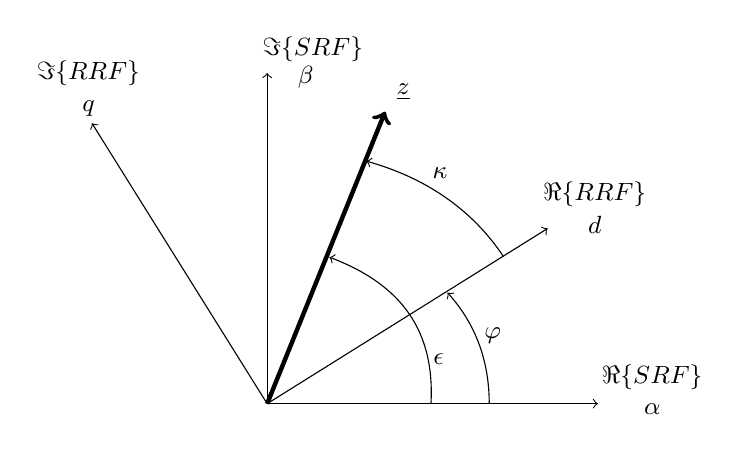
\begin{tikzpicture}[
    axis/.style={->, thick},
    vector/.style={->, very thick},
    angle/.style={->, thick},
    every node/.style={font=\small}
]


\def\R{4.2}        % length of reference axes
\def\angRRF{32}    % phi: RRF rotation relative to SRF
\def\angZ{68}      % epsilon: z angle relative to alpha axis
\def\Vz{4.0}       % magnitude of z


\coordinate (O) at (0,0);

\coordinate (A) at (\R,0);
\coordinate (B) at (0,\R);

\draw[axis, thin] (O) -- (A)
;

\draw[axis, thin] (O) -- (B)
;
\coordinate (D) at ({\R*cos(\angRRF)},{\R*sin(\angRRF)});
\coordinate (Q) at ({\R*cos(\angRRF+90)},{\R*sin(\angRRF+90)});

\draw[axis, thin] (O) -- (D)
;

\draw[axis, thin] (O) -- (Q)
;


\coordinate (Z) at ({\Vz*cos(\angZ)},{\Vz*sin(\angZ)});

\draw[vector, ultra thick, ->] (O) -- (Z)
    node[at end, above right] {$\underline{z}$};


\coordinate (Zd) at
    ({\Vz*cos(\angZ)*cos(\angRRF) +
      \Vz*sin(\angZ)*sin(\angRRF)},
     {(\Vz*cos(\angZ)*cos(\angRRF) +
      \Vz*sin(\angZ)*sin(\angRRF))*sin(\angRRF)});

\node at (0.58,4.5) {$\Im\{SRF\}$};

\node[align=center] at (2.23,0.57) {
    $\epsilon$
};
\node[align=center] at (2.92,0.87) {
    $\varphi$
};
\node[align=center] at (2.25,2.93) {
    $\kappa$
};


  \node at (-2.27,4.19) {$\Im\{RRF\}$};

  \node at (4.89,0.34) {$\Re\{SRF\}$};

  \node at (4.16,2.66) {$\Re\{RRF\}$};
  \draw[->] (2.08,0) .. controls (2.13,0.91) and (1.72,1.51) .. (0.79,1.86);

  \draw[->] (2.82,0) .. controls (2.82,0.54) and (2.65,1.01) .. (2.29,1.41);
  \draw[->] (3,1.87) .. controls (2.6,2.47) and (2.01,2.87) .. (1.26,3.08);

  \node[align=center] at (4.89,-0.07) {$\alpha$};

  \node[align=center] at (0.49,4.15) {$\beta$};

  \node[align=center] at (4.16,2.27) {$d$};

  \node[align=center] at (-2.27,3.75) {$q$};
\end{tikzpicture}
